\documentclass[10pt,a4paper,bibliography=totoc,twocolumn]{scrartcl}
\usepackage[ngerman]{babel}
\usepackage[utf8]{inputenc}
\setlength{\parskip}{1em}
\setlength{\parindent}{1em}
\usepackage{hyperref}
\usepackage{mathtools}
\usepackage[numbers]{natbib}
\usepackage{url}
\usepackage{algpseudocode}
\usepackage{algorithm}
\usepackage{listings} 
\usepackage{amssymb}
\usepackage{graphicx}
\usepackage{amsmath}
\usepackage[normalem]{ulem}
\usepackage{soul}
\usepackage{color}
\usepackage[table,xcdraw]{xcolor}
\usepackage{pdflscape}
\usepackage{booktabs}
\usepackage{longtable}
\usepackage{geometry}
\usepackage[T1]{fontenc}% wichtig für Trennung von Wörtern mit Umlauten
\usepackage{microtype}% verbesserter Randausgleich
\usepackage[toc,page]{appendix}
\usepackage[all]{nowidow}
\usepackage[style=base, margin=5mm]{caption}
\usepackage{siunitx}
\geometry{a4paper,left=16mm,right=16mm, top=25mm, bottom=3cm} 
\setlength{\columnsep}{16pt}
\DeclareMathOperator*{\argmax}{arg\,max}
\DeclareMathOperator*{\counti}{count}

\begin{document}


\title{Methoden zur automatischen Farbkonfiguration von Weboberflächen aus Bildvorlagen}
\subtitle{Masterproject Zwischenabgabe I}
\author{Philipp Anders}

\twocolumn[
  \begin{@twocolumnfalse}
    \maketitle
    \begin{abstract}
Ziel des Projekts ist die automatische Farbkonfiguration der Oberflächenelemente von Webseiten (Text, Buttons, Hintergründe, etc.) aus Bildvorlagen. Dabei wird das Problem in zwei Teilprobleme zerlegt: 1. Das Bilden einer Obermenge von Farben durch einen Algorithmus zur Color Palette Estimation (CPE). 2. Die Identifizierung von Farben für bestimmte Oberflächenelemente aus dieser Obermenge durch Lösung eines Constraintsystems. Für die CPE wird der ACoPa-Algorhitmus von \citet{acopa} ausgewählt und implementiert, da dessen Ergebnis den aus Styleguides bekannten Farbpaletten-Definitionen in Form von Color Swatches ähnelt.
  \vspace*{1cm}
    \end{abstract}
  \end{@twocolumnfalse}
]

\section{Einleitung}

\subsection{Problemmodellierung}
\label{sec:modellierung}

Der CSS-Standard zur Beschreibung des Erscheinungsbildes von Webseiten definiert mehr als 10 Eigenschaften zur farblichen Gestaltung von Texten, Hintergründen, Tabellen und anderen HTML-Elementen \citep{css3-color}. Ziel dieser Arbeit ist die automatisierte Bestimmung der Farbwerte von Elementen in Webseiten. Betrachtet werden all jene Oberflächenelemente, die visuell als Blöcke wahrgenommen werden (d.h. die Hintergrundfarbe \texttt{"background-color"} von \texttt{<div>}, \texttt{<button>}, \texttt{<p>} etc.) , sowie Texte (d.h. die Vordergrundfarbe \texttt{"color"} der Blöcke sowie von \texttt{<h1>}, \texttt{<a>}, etc.). Ziel ist also die Farbbestimmung von \textbf{Blöcken} und \textbf{Texten}, Rahmen und andere Textdekoration werden dabei ignoriert.

Üblicherweise werden mehrere Elemente eines HTML-Dokuments auf die gleichen Farben abgebildet. Beispielsweise können alle Links (Textfarbe) sowie Buttons (Hintergrundfarbe) die gleiche Farbe erhalten. Im Folgenden wird eine Menge von Elementen einer Webseite mit gleicher Farbabbildung als \textbf{Color Group} $CG$ bezeichnet \citep[siehe auch][]{webpage, patterns}. Die Menge aller Color Groups einer Webseite wird als $CGs$ formalisiert. Dabei gilt $|CGs| = k$, eine Webseite beinhaltet also $k$ Color Groups. Abbildung \ref{fig:colorgroups} veranschaulicht dies anhand einer exemplarischen Webseite für Musikstreaming, welche sieben Color Groups beinhaltet.

Als vorbereitender Schritt wird der Suchraum zur Identifizierung geeigneter Farben durch die Zusammenstellung einer sogenannten \textbf{Farbpalette} verkleinert \citep{webpage}. Dabei handelt es sich um eine Farbmenge $P = \{c_1, c_2, \ldots, c_n\}$ mit $n$ Farben, wobei jedes $c \in P$ als String von RGB Werten kodiert wird. Formal ist damit das Ziel dieser Arbeit die Ermittlung einer Abbildung $CGs \to P$. Die Abbildung muss injektiv sein, d.h. nicht jede Farbe der Farbpalette $P$ muss verwendet werden, jedoch dürfen mehrere Color Groups nicht gleich gefärbt werden. Es gilt $k \leq n$.

Entscheidendes Kriterium für die Zuordnung ist eine funktionale Gestaltung der Webseite. Im Rahmen dieser Arbeit wird hierunter eine Farbgestaltung verstanden, die Accessibility (Lesbarkeit) und Usability (Benutzerfreundlichkeit) gewährleistet. Eine intuitiv widersinnige Färbung ist beispielsweise ein roter Text auf orangem Hintergrund mit grauem Button. Weder ist der Text lesbar (Accessibility), noch wird die Aufmerksamkeit des Nutzers auf das Interaktionselement gelenkt (Usability). 

Als Besonderheit dieser Arbeit soll die Farbpalette P auf einer Bildvorlage basieren. So wird eine Harmonisierung des visuellen Eindrucks einer Weboberfläche und der darin enthaltenen Grafik erreicht. Da die gewählte Farbgebung wesentlich für die vermittelte Atmosphäre einer Webseite ist \citep{webdesign}, soll die Anpassung der Farbgebung an ein Motiv dessen Eindruck unterstützen. Da die Farbpalette somit auf den verarbeiteten Daten basiert, ist eine Berechnung zur Laufzeit möglich, wenn ein effizientes Suchverfahren ermittelt wird. Ein Anwendungsbeispiel hierfür ist die farbliche Anpassung einer Seite für Musikstreaming an das gespielte Albumcover. Abbildung \ref{fig:colorgroups} zeigt hierfür ein Gegenbeispiel: keine der Farben des Cover taucht in der umgebenen Weboberfläche auf.

\begin{figure}[h]
	\centering
	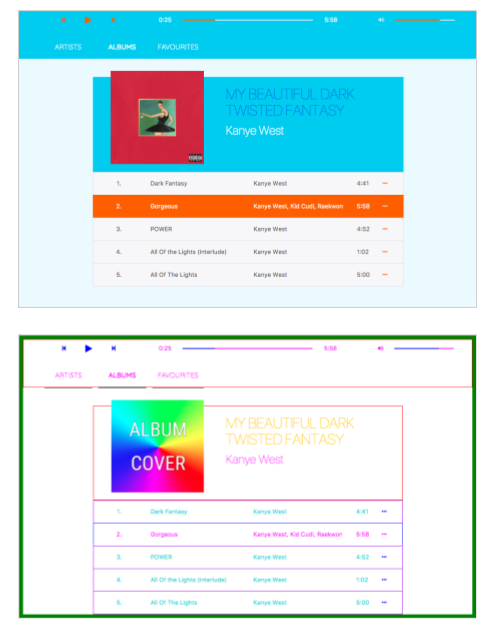
\includegraphics[width=0.48\textwidth]{img/color_groups.png}
	\caption{Beispiel der Farbgestaltung einer exemplarischen Weboberfläche für Musik-Streaming. Oben: Originales Farbdesign. Unten: Hervorhebung der sieben Color Groups. Elemente einer Color Group erhalten die gleiche Farbe. Blöcke sind umrahmt.}
	\label{fig:colorgroups}
\end{figure}

\subsection{Color Palette Estimation}

Die Zusammenstellung einer Farbpalette aus einer Bildvorlage wird von \citet{acopa} als \textbf{Color Palette Estimation (CPE)} bezeichnet und als die Repräsentation eines Bildes mit einer minimalen Menge von Farben beschrieben. Diese ist dann minimal, wenn redundante Farben reduziert und die seltenen Farben der für die Wahrnehmung wichtigen Objekte erhalten bleiben. Formale Kriterien werden von den Autoren jedoch nicht geliefert. Abbildung \ref{fig:ladybug} veranschaulicht diese intuitive Definition am Beispiel eines Bildes mit einem Marienkäfer, dessen Sichtbarkeit von der Wahl der Farbpalette abhängt.

\begin{figure}
\centering
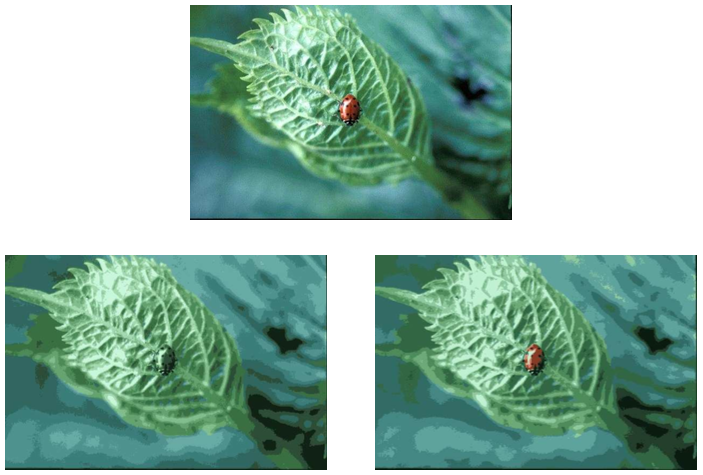
\includegraphics[width=0.48\textwidth]{img/ladybug.png}
\caption{Beispiel für die Einfärbung eines Bildes mit unterschiedlichen Farbpaletten der Größe 12. Oben: Originalbild. Links: Farbpalette ohne rote Farbtöne. Rechts: Farbpalette mit roten Farbtönen, wodurch der Marienkäfer erkennbar ist (Quelle: \citep{acopa})}
\label{fig:ladybug}
\end{figure}

Historisch geht die CPE aus der Farbquantisierung hervor, bei der die Farben von Grafiken aufgrund der damals zu kleinen Kapazität von Grafikpuffern vor deren Anzeige reduziert (Farbreduktion) und dann auf die reduzierte Farbpalette abgebildet werden mussten (Quantisierung) \citep{variance}. Aus diesem Kontext kommt das formale Kriterium der Summe des quadratischen Fehlers, welcher in diesem Anwendungsfall auch als \emph{Recoloring Error} bezeichnet wird \citep{colorthemes}.

Da Grafikpuffer mittlerweile über ausreichend Kapazität verfügen, liegt die Anwendung der CPE in anderen Bereichen wie z.B. der farbbasierten Indizierung von Grafiken in Datenbanken oder der Zusammenstellung von Farbthemen zu Gestaltungszwecken. \citet{colorthemes} zeigen, dass in diesem Kontext der Recoloring Error keine geeignete Metrik zur Beurteilung der Güte einer Farbpalette in Bezug auf das Ausgangsbild ist. Grund sind die menschlichen Wahrnehmungseigenschaften, wobei Bilder auf Komponenten- und nicht auf Pixelebene erfasst werden. Stattdessen werden eine Reihe anderer Metriken vorgestellt, die diesen Umstand berücksichtigen. Die Autoren zeigen zusätzlich empirisch, dass abhängig vom Individuum ein und dieselbe Farbpalette eines Bildes für unterschiedlich repräsentativ gehalten wird. 

Dieser Befund hebt hervor, dass die Güte einer Farbpalette in Bezug auf das Ausgangsbild subjektiv ist und vom Anwendungsbezug abhängt. Aus diesem Grund wird für die Güte der zu ermittelnden Farbpalette $C$ keine objektive Bewertungsfunktion herangezogen. Stattdessen wird die Farbpalette in Hinblick auf ihre Zweckmäßigkeit zur farblichen Gestaltung einer Webseite bewertet. Das heißt, die aus der Grafik hervorgehende Farbpalette muss eine Teilmenge an Farben beinhalten, mit welcher die automatisierte Farbgestaltung einer Webseite lösbar ist. Hierfür müssen Kriterien abgeleitet, indem Prinzipien für eine Funktionale Gestaltung von Webseiten sowie Farbdefinitionen aus Style Guides analysiert werden. Davon ausgehend wird eine geeignete Herangehensweise zur Bestimmung einer solchen Farbpalette aus einer Bildvorlage ermittelt.

\section{Einordnung und Literaturbesprechung}

Damit Arbeit ordnet sich in das Gebiet automatisierten Farbgestaltung (\textbf{Color Design Automation}) ein. In diesem Bereich hat in den letzten Jahren Forschung in verschiedenen Anwendungsbezügen stattgefunden, wobei überwiegend Methoden des maschinellen Lernens zur Problemlösung eingesetzt wurden.

\citet{colorcomp} haben 2011 eine Grundlage für spätere Systeme zur automatisierten Farbgestaltung gelegt, indem sie ein Regressionmodell zur Bewertung der Ästhetik von Farbpaletten der Größe 5 entwickelten. Hierfür wurde in Training an den Datenbeständen von Farbpaletten-Communities wie z.B. Adobe Color\footnote{\url{https://color.adobe.com/de/explore/}} durchgeführt. Dabei hat sich unter anderem ergeben, dass die auf geometrischen Strukturen im Farbkreis beruhenden Modelle der klassischen Farbentheorie nicht zur Vorhersage von Farbhamonie geeignet sind. Hierzu zählen zum Beispiel die Farbton-Schablonen von \citet{itten} oder \citet{munsell}. Dies ist insofern bemerkenswert, als dass diese Modelle in zahlreichen Unterstützungswerkzeugen zur Farbgestaltung ihre Umsetzung finden. Die Grenzen des trainierten Modells liegen in der Bewertung der Harmonie von Farben im tatsächlichen Anwendungskontext, da die Auswirkungen der räumlichen Ausprägung von Farben nicht überprüft werden \citep{webpage, patterns}. Eine Matlab-Implementierung des Modells zur Überprüfung von Farbharmonien steht öffentlich zum Download bereit \footnote{\url{http://www.dgp.toronto.edu/~donovan/color/}}.

\citet{patterns} haben sich 2013 mit einer Lösung für eine sehr grundlegende Form für ein Färbungsproblems auseinandergesetzt: Die Kolorierung von Mustern nach dem Prinzip "Malen nach Zahlen". Hierfür wurde ein probabilistisches Modell entwickelt, indem über 8000 von Künstlern entworfene Muster von der Seite \url{http://www.colourlovers.com/} ausgewertet wurden. Eine vorgeschlagene Anwendung stellt die Umkehrung des Ziels dieser Arbeit dar: Die Anpassung eines Musters an das Farbschema einer Webseite. Die Autoren stellen Eigenschaften zur Bestimmung von Hintergrund- und Vordergrundfarben sowie zur Kontrastberechnung vor, die für diese Arbeit genutzt werden können. Zur Lösungssuche wird \emph{Factor Graph} modelliert, welcher ebenfalls ein Ansatz für die vorliegende Arbeit darstellt. Das Modell von \citet{colorcomp} wird als externer Bestandteil des Graphen hinzugefügt, um eine globale Kompatibilität der eingesetzten Farben zu gewährleisten.

\citet{webpage} haben sich 2016 mit der automatisierten Farbgestaltung von Webseiten. Durch die Auswertung von 500 Webseiten wurde ein probabilistisches Modell als Optimierungsproblem mit mehreren Zielen formuliert. Eine der Zielfunktionen gewährleistet ausreichenden Kontrast zwischen den Webelementen. Eine andere Zielfunktionen passt die Farbgestaltung an ein Schlüsselwort an (z.B. \emph{Business} oder \emph{Fresh}). Die letzte Zielfunktion gewährleistet Farbharmonie, was wiederum durch das Modell von \citet{colorcomp} implementiert wird. Die Optimierung wird durch eine lexikographische Strategie realisiert, bei welcher in Interaktion mit einem Gestalter die Zielfunktionen nacheinander angewendet werden. In einer Anwendung extrahieren die Autoren ebenfalls eine Farbpalette aus einer Grafik und nutzen diese als Grundlage zur Färbung der Webseite. Zur CPE wurde der K-Means Algorithmus verwendet. Im Gegensatz zum Gegenstand dieser Arbeit erfordert der vorgestellte Prozess jedoch eine Nutzerinteraktion aufgrund der lexikographischen Strategie. Somit handelt es sich eher um ein Unterstützungswerkzeug für Gestalter und kein System zur automatisierten Bestimmung einer Farbgestaltung zur Laufzeit. Die Autoren stellen eine Systemarchitektur vor, welche als Grundlage für die vorliegende Arbeit adaptierbar ist.

\citet{magazines}  haben sich 2013 mit der automatisierten Farbgestaltung von Magazin-Covers auseinander gesetzt. Vergleichbar mit \citep{webpage} wird auch hier die Optimierung des Farbkontrasts, der Farbharmonie und der Farbsemantik verfolgt.  Im Gegensatz zu den bisherigen Lösungen wird hier allerdings mit expliziten Modellen anstatt mit Trainingsdaten gearbeitet. Über Flowcharts vermitteln die Autoren Lösungsprozeduren zur Suche geeigneter Schriftfarben und Stellen konkrete Grenzwerte vor, die für diese Arbeit übernommen werden können.

\section{Problemlösungansatz und Systemarchitektur}

Ausgehend von der Literaturbesprechung wird ein Ansatz zur Problemlösung besprochen. Darauf aufbauend wird eine konkrete Architektur des zu implementierenden Systems entwickelt. Im Hauptteil werden für die einzelne Bestandteile der Architektur geeignete Methoden besprochen und ausgewählt.

Es ist ein Modell zu entwickeln, welches die Abbildung $CGs \to P$ beschreibt. \citet{webpage} stellen für die automatisierte Farbgestaltung zwei grundlegende Herangehensweisen vor:

\begin{enumerate}
	\item \textbf{Regelbasiert:} Beschreibt quantitative Modelle mit determinstischem Regelwerk. Die Arbeit von \citet{magazines} stellt hierfür ein Beispiel dar. Durch die Analyse von Farbharmonie-Modellen wurden Regeln für die automatisierte Gestaltung abgeleitet.
	\item \textbf{Datengetrieben:} Beschreibt Modelle, welche die Performanz möglicher Lösungen einer automatisierten Farbgestaltung auf Grundlage existierender Beispieldaten vorhersagt.
\end{enumerate}

Die regelbasierten Modelle treffen präzise Aussagen im Gegensatz zu probabilistischen Modellen, tendieren jedoch zur zu starken Abstraktion vom Anwendungskontext. Im Gegensatz dazu stützen sich die Modelle des datengetriebenen Ansatzes auf reale Daten und tendieren daher zu robusteren Ergebnissen in der Anwendungsdomäne \citep{webpage}. Da bei den probabilistischen Modellen potentielle Lösungen bewertet und gegeneinander abgewogen werden müssen, sind hohe Laufzeiten möglich. Die bereits entwickelte Lösung von \citet{webpage} zur automatisierten Farbgestaltung von Websites benötigt selbst nach Optimierung des Suchverfahrens 2 Stunden zur Konvergenz. Außerdem ist deren vorgestellter Prozess zur Anpassung der Farbgestaltung einer Webseite an nicht im eigentlichen Sinne vollautomatisch: Einerseits erfordert die Verwendung des K-Means Algorithmus zur CPE die Bestimmung der Farbanzahl (k) vom Gestalter, andererseits erfordert die lexikographische Strategie einen Nutzerinteraktion während des Optimierungsprozess.

Aus diesen Gründen wird sich diese Arbeit auf einen \textbf{regelbasierten} Ansatz \textbf{ohne Nutzerinteraktion} konzentrieren, d.h. vollautomatisiert. Auch ohne die Auswertung großer Datenmengen existieren quantitative Modelle, um die Accessibility einer Webseite zur gewährleisten. Beispielsweise geben die \emph{Web Content Accessibility Guidelines} \citep{wcag} quantitative Grenzwerte für die Lesbarkeit von Text an. Es sind Eigenschaften und Bedingungen zu erarbeiten, die für Farben einzelner Color Groups sowie zwischen diesen gelten sollen. Diese Einschränkungen werden im Folgenden als \textbf{Constraints} bezeichnet. Ein System von Constraints mit endlichem Wertebereich (in diesem Fall $P$) wird als \textbf{Constraint Satisfaction Problem} (CSP) bezeichnet \citep{constraint-programmierung}. \citet{magazines} haben gezeigt, dass eine Lösung eines solchen Constraint-Systems beispielsweise über Faktor-Graphs möglich ist.

Nicht jede Webseite hat die gleiche Anzahl Color Groups. Um die Komplexität des Constraint-Systems zu reduzieren, wird auf die Feststellung der Color Groups einer Webseite verzichtet. Stattdessen wird von einer Webseite als Layout \textbf{abstrahiert}. Ein Layout definiert, welche Color Groups mit welcher Semantik existieren. Beispielsweise definiert ein Layout eine Color Group, welche alle Buttons beinhaltet und deren Semantik \emph{Interaktion} ist. Aus Sicht des Constraint-Systems werden keine Farben für einzelnen Buttons, sondern eine Interaktionsfarbe gesucht. Durch das Konzept der Color Groups wird also von den betreffenden Elementen abstrahiert.

Zur Lösungssuche mit einem regelbasierten Ansatz existieren zwei Herangehensweisen:
\begin{enumerate}
    \item \textbf{Constraints-First}: Setze $n = k$. Hierbei wird die Lösungssuche zum Zeitpunkt der CPE verlagert. Unter Kenntnis der Color Groups ist hier der Suchraum das Histogram der Bildvorlage. Dieser Ansatz wird unter anderem von \citet{colorcomp} verfolgt. Sie verwenden ihr Regressionsmodell zur Bewertung der Farbharmonie, um eine alternative Optimierungsfunktionen zur Suche von $P$ im Farbraum einer Bildvorlage zu formulieren.
    \item \textbf{Constraints-Last}: Setze $k \leq n$. $P$ wird unabhängig vom Layout ermittelt. Der Suchraum beschränkt sich dann auf die Farben in $P$. Dieser Ansatz wird unter anderem von \citet{documentpalette} bei der automatisierten Farbgestaltung von Dokumenten verfolgt. Nach der Bestimmung einer Farbpalette aus einer Bildvorlage werden sukzessive geeignete Farben aus $P$ ausgewählt. Zuerst wird die Hintergrundfarbe komplementär zum Hintergrund des Bildes gewählt, welche via Bildsegmentierung bestimmt wurde. Daraufhin wird die Textfarbe unter Beachtung des Kontrastes aus $P$ gewählt.
\end{enumerate}

Für diese Arbeit wird die Herangehensweise \textbf{Constraints-Last} bevorzugt. Sie beinhaltet die Aufteilung des Problems in zwei getrennte Suchverfahren: Ein Suchverfahren für die Bestimmung von $P$ und ein Suchverfahren zur Bestimmung der Abbildung $CGs \to P$. Dadurch wird eine Wiederverwendung einmal bestimmter Farbpaletten für verschiedene Layouts ermöglicht. Für die Arbeit bedeutet dies, dass eine Problemlösung anhand eines exemplarischen Layouts mit bestimmten Color Groups gezeigt wird, eine Übertragung auf andere Layouts jedoch möglich ist. Schlussendlich ermöglicht ein Cashing bereits berechneter Farbpaletten das Einsatzpotential der automatisierten Farbgestaltung zur Laufzeit.

Selbst unter den gegebenen Einschränkung des Suchraums durch die vorgeschaltete Ermittlung einer Farbpallete ist die Menge potentieller Lösungen mit $\binom{n}{k} k!$ nach wie vor groß. Für die exemplarischen Werte $|CGs| = k = 5$ und $|P| = n = 10$, d.h. 5 Colorgroups (z.B. Text, Texthintergrund, Buttons, Navigations-Hintergrundfarbe und Footer-Hintergrundfarbe) sowie eine Farbpalette mit 10 Farben, ergeben sich $\binom{10}{5} 5! = 30.240$ mögliche Kombinationen. Es ist ein effektives Suchverfahren zur Ermittlung von $CGs \to P$ zu identifizieren. Die bereits vorgestellte hierarchische Ansatz von \citet{documentpalette} stellt hierfür einen Ansatz dar, bei welchem wichtige Farbzuordnungen zuerst getroffen werden und dadurch der Suchraum für folgende Color Groups eingeschränkt wird (z.B. erst Hintergrund, dann Textfarbe).

\begin{figure*}
	\centering
	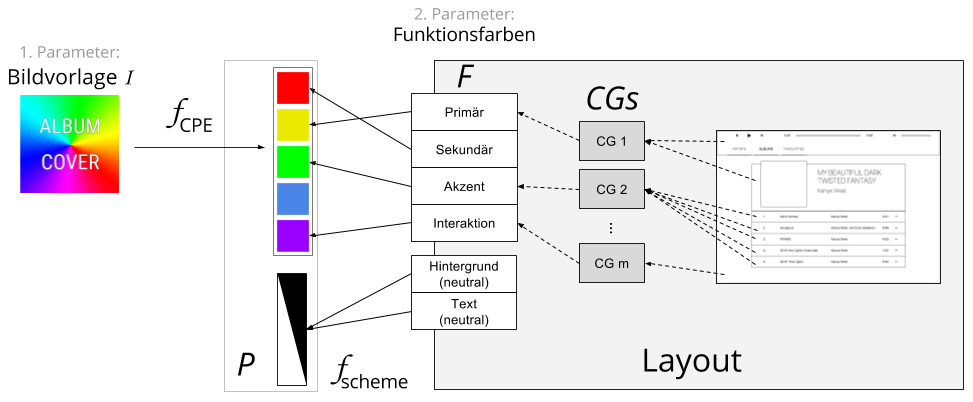
\includegraphics[width=1\textwidth]{img/architecture.png}
	\caption{System-Architektur. Der grau unterlegte Kasten visualisiert den Bereich, für den algorithmische Lösungen gefunden werden müssen. Die Eingabeparameter sind eine Bildvorlage und eine Menge von Color Groups, welche von einem Layout definiert werden. Das System setzt zwei Suchverfahren um, welche mit $f1$ und $f2$ bezeichnet werden. $f1$ ermittelt zuerst eine Farbpalette aus der Bildvorlage (CPE).  $f2$ ordnet Colour Groups Farben aus der Palette, in dem ein entsprechendes Constraint System gelöst wird. Nachdem eine Farbabbildung gefunden wurde, wird das kolorierte Layout ausgegeben. }
	\label{fig:architecture}
\end{figure*}

\subsection*{Zusammenfassung}

Abbildung \ref{fig:architecture} fasst den Ablauf der automatisierten Farbgestaltung einer Webseite zusammen. Das zu entwickelnde System bildet eine Bildvorlage auf eine Farbpalette ab. Das Suchverfahren hierfür wird was als Color Palette Estimation (CPE) bezeichnet. Die entstandene Palette wird zum Suchraum für die Color Groups, welche durch ein Layout definiert werden. Da bei dieser Abbildung der Wertebereich einer Color Group auf die Elemente der Farbpalette beschränkt ist, handelt es sich um ein Constraint Satisfaction Problem (CSP). Letztendlich wird eine kolorierte Variante des Layouts ausgegeben.

Im Folgenden sind konkrete Verfahren für die beiden Teilprobleme CPE und CSP zu ermitteln. 


\subsection{Farbpaletten in Style Guides}
\label{sec:swatches}

Style Guides zur Oberflächengestaltung beinhalten unter anderem Richtlinien für den Farbeinsatz. Dabei werden i.d.R. eine Obermenge von Farben definiert und mit Verwendungshinweisen verbunden. Einige Farben, wie z.B. die Logo-Farbe, stehen hierbei unter strikten Restriktionen. Davon abgesehen wählt der Designer eine Untermenge von Farben der Farbpalette aus dem Style Guide und legt selbst Einsatzregeln fest, wie z.B. die Farbe für Interaktionselemente.

Die Apple \emph{iOS Human Interaction Guidelines} legen eine Farbpalette von 8 strahlenden Farben fest, die sich aufgrund ihrer Intenstität ausschließlich für Interaktionselemente und ausgewählte Komponenten wie z.B. Statusleisten eignen \citep{ios}. Demgegenüber beschreibt Google im \emph{Material Design Style Guide} Farben in Form eines Farbtons in abgestuften Schattierungen. Dieses Konzept wird als \emph{Color Swatch} bezeichnet. Hierbei handelt es sich um ein Erweiterung der Farbpalette, die dem Designer mehr Spielraum bei der farblichen Komposition einräumt. Ein Beispiel hierfür zeigt Abbildung \ref{fig:swatches}, auf welcher ein Auszug der Color Swatches und ein Einsatzbeispiel für den Umgang mit Schattierungen gezeigt wird. Ein anderes Beispiel hierfür zeigt das Corporate Design Hanbuch der HTWK Leipzig. Der Farb-Guide stellt Color Swatches mit zwei bis drei Schattierungen bereit \citep{htwk}.

Das Konzept der Color Swatches wird in dieser Arbeit für die CPE bevorzugt, da über die Farbeigenschaften eines Bildes keine Annahmen getroffen werden können. Die Bereitstellung eines Farbtons in verschiedenen Schattierungen ermöglicht jedoch den flexiblen Einsatz von Farben, der bei Bildern mit wenig Farben notwendig ist. So ist z.B. der selbe Farbton sowohl für Interaktionselement, oder in einer hellen Schattierung für den Hintergrund einsetzbar. 

\begin{figure}[h]
	\centering
	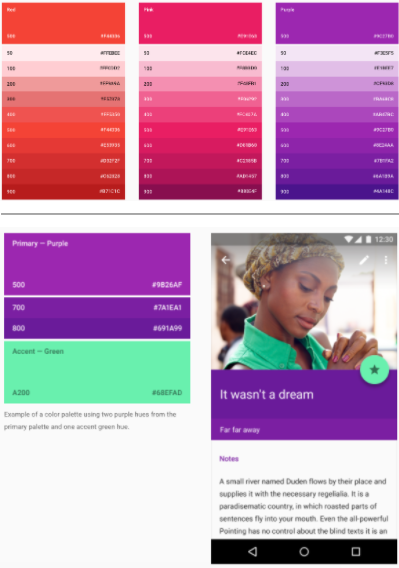
\includegraphics[width=0.48\textwidth]{img/material_design.png}
	\caption{Auszug der Color Swatches in der Farbpalette des Google Material Designs (oben) mit Einsatzbeispiel (unten). (Quelle: \citep{google})}
	\label{fig:swatches}
\end{figure}

\section{Algortihmen zur Color Palette Estimation}

Im Folgenden wird eine Algorithmus zur Lösung des Teilproblems der Ermittlung der Farbobermenge $C_s$ gesucht. Hierzu findet eine Betrachtung von Typen vorhandener Algorithmen zur CPE statt. Abschließend wird ein geeigneter Algorithmus ausgewählt

\subsection{Überblick}

Grundlegend sind zwei Ansätze zur CPE zu unterscheiden:
\begin{enumerate}
    \item \textbf{Hisgoram-basiert}: Algorithmen, die nur auf dem Histogramm des Bildes arbeiten und somit die Positionsinformationen der Farben nicht beachten. Es handelt sich (bis auf Ausnahmen) um Clustering-Verfahren, die durch eine Partitionierung des Farbraums Gruppen ähnlicher Farben im Histogramm identifizieren.
    \item \textbf{Bildsegmentierungs-basiert}: Algorithmen, die durch eine Segmentierung des Bildes zunächst zusammenhängende Komponenten identifizieren und für diese dann repräsentative Farben identifizieren.
\end{enumerate}


Bildsegmentierungs-basierte Algorithmen berücksichtigen die menschlichen Wahrnehmungseigenschaften auf Komponentenebene, führen aber durch die zusätzliche Betrachtung der Positionsinformation eine weitere Komplexitätsebene ein \citep{colorthemes}.

\citet{categorization} treffen eine Kategorisierung der Histogramm-basierten Verfahren in \emph{hierarchisch} und \emph{iterativ}. Hierarchisch arbeitende Algorithmen zur CPE werden auch als \emph{Pre-Clustering Verfahren} bezeichnet, da sie vor dem Erreichen der (fest zu wählenden) Farbanzahl $n$ mit mehr bzw. weniger Farben starten. Sie basieren auf der statistischen Analyse der Verteilung der Bildfarben im Farbraum. In diese Kategorie fallen \emph{top-down} bzw. \emph{bottom-up} Clustering-Algorithmen. Zu den Top-Down Verfahren zählen die in der Vergangenheit populären Raumunterteilungs-Algorithmen wie z.B. Mediancut \citep{mediancut} oder Octree\citep{octree}. Sie Zerteilen den Farbraum sukzessiv in disjunkte Teilräume und unterstellen den Clustern dabei eine Würfelform. Ergebnis der Verarbeitung ist ein Dendogram, wobei die Blätter die Farben Farbpalette repräsentieren. Ein Schnitt des Dendograms entspricht einer Partitionierung des Raums, welche jedoch auch direkt durch die iterativ arbeitenden Algorithmen erreichbar ist \citep{acopa}. Diese Verfahren werden darum auch als \emph{partitionierend} \citep{acopa} oder auch \emph{Post-Clustering} \citep{categorization} bezeichnet. Sie starten bereits mit der erforderlichen Anzahl Farben $n$ und verbessern diese iterativ. Einige Methoden dieser Klasse verwenden den quadratischen Fehler, wie z.B. K-Means \citep{kmeans, kmeanshsi} oder Fuzzy C-Means \citep{fuccycmeans}. Andere analysieren das Histogramm auf dichte bzw. weniger dichte Regionen, wie z.B. Mean-Shift \citep{meanshift}. Eine detailliertere Vorstellung von Algorithmen zur CPE bietet \citep{categorization2}.

\begin{figure}[h]
\centering
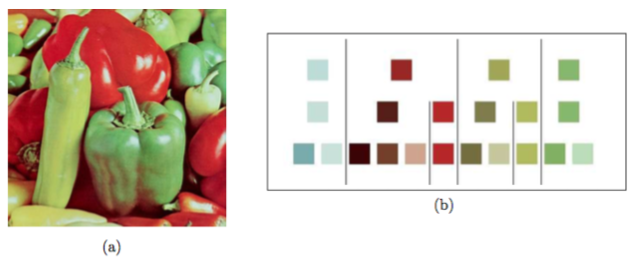
\includegraphics[width=0.48\textwidth]{img/peppers.png}
\caption{CPE Ergebnis von ACoPa. (a) Originalbild "Peppers" (b) Hierarchische Farbpalette. Die unterste Ebene zeigt die finalen Farben. (Quelle: \citep{acopa})}
\label{fig:peppers}
\end{figure}

\citet{acopa} kritisieren an den bisherigen Algorithmen, dass die Anzahl gesuchten Farben $n$ zuvor bekannt sein muss, dass die Ergebnisse abhängig von der Initialisierung sind und dass Farben kleiner Bilddetails im Sinne der Definition in Abschnitt \ref{sec:modellierung} nur unzureichend repräsentiert werden, wie im Paper experimentell nachgewiesen wird. Aus diesem Grund stellen sie den \textbf{Automatic Color Palette (ACoPa)} Algorithmus vor, welcher durch die Analyse von Spitzen des Histogramms im HSI Raums eine Farbpalette erstellt und dabei deren Größe selbstständig bestimmt. Der Algorithmus ermittelt dabei zunächst die grundlegenden Farbtöne (Hue) des Bildes und schlüsselt diese daraufhin sukzessive nach deren Sättigungen (Saturation) und Schattierungen (Intensity) auf. Abbildung \ref{fig:peppers} veranschaulicht exemplarisch die hierarchische Arbeitsweise, bei der in jeder Ebene zusätzliche Sättigungen und Schattierungen der enthaltenen roten und grünen Farbtöne gebildet werden.

\subsection*{Zusammenfassung und Wahl des Algorithmus zur CPE}

Der Algorithmus zur CPE soll eine Obermenge $C_s$ von Farben bilden, aus welcher im einem nachfolgenden Schritt eine Teilmenge von Farben $C$ entsprechend ihrer Eignung für bestimmte Oberflächenelemente ausgewählt werden. Analog dazu werden Farbpaletten in Styleguides als Obermenge von Farben beschrieben, aus welcher der Designer eine Untermenge von Farben für die konkrete Oberfläche auswählt. Bestimmte Styleguides erweitern dabei das Farbpalettenkonzept um Color Swatches, bei welchen Farbtöne in zusätzliche Schattierungen aufgefächert werden. Dadurch hat der der Designer eine größere Flexibilität beim Einsatz der Farbpalette.

Aus diesen Gründen wird der ACoPa Algorithmus von \citet{acopa} zur CPE gewählt.Da er Farbwerte automatisch in verschiedenen Sättigungen und Schattierungen ermittelt, imitiert er die Farbdefinition in Form von Color Swatches in Styleguides. Durch seine parameterfreie Arbeitsweise ermittelt er selbstständig die Anzahl repräsentativer Farben im Bild. Dadurch wird automatisch die erforderliche Obermenge zur Bildung der finalen Farbpalette bereitgestellt, wenn das Bild ausreichend viele Farben enthält. Das erzwingen eines großen Farbpalette mit anderen Clusteringverfahren, z.B. über einen pauschal großen K Parameter bei K-Means, führt hingegen unter Umständen zu einer Partitionierung des Farbraums, die nicht der Clusterstruktur des Histogramms entspricht.

\section{ACoPa}

Im Folgenden wird die grundlegende Arbeitsweise des ACoPa Algorithmus nach \citet{acopa} vorgestellt. Dabei werden die Herausforderungen, die bei der Implementierung aufgetreten sind, besprochen. Abschließend werden exemplarisch Anwendungsergebnisse präsentiert.

\subsection{Konvertierung in den HSI-Raum}

\begin{figure*}
\centering
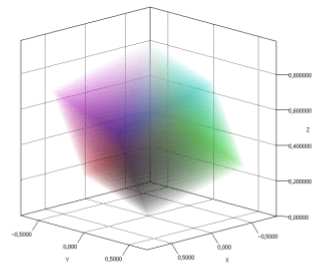
\includegraphics[width=1\textwidth]{img/hsi_conversion.png}
\caption{Gegenüberstellung von RGB zu HSI-Umrechungsergebnisse. (a.) Referenz-HSI Raum. (b.) Umrechnung nach \citep{acopa}. (c.) Umrechnung nach \citep{colorimage}.}
\label{fig:hsi_conversion}
\end{figure*}

Zunächst wird das Histogram in den HSI Farbraum $\{(h, s, i) \ | \ 0 \leq h < 360 \wedge 0 \leq s, i \leq 1\}$ übertragen. Die Intensität eines Farbtons wird dabei in Polarkoordinaten via $h$ und $s$ angegeben, während die maximal mögliche Sättigung wiederum von der Intensität $i$ abhängt. Zur Konvertierung vom RGB in HSI Raum wurden verschiedene Umrechnungsvorschriften erprobt. Die Umrechnung gemäß der ACoPa-Autoren lautet:

\begin{equation}
\begin{split}
I = \frac{R+G+B}{3} \\
S = \sqrt{(R-I)^2 + (G-I)^2 + (B-I)^2} \\  
H = \arccos{(\frac{(G-I)-(B-I)}{S\sqrt{2}})}
\end{split}
\label{eq:hsi_acopa}
\end{equation}

Die Umrechnung gemäß eines Lehrbuchs für Farbbild-Verarbeitung \citep{colorimage} lautet hingegen:

\begin{equation}
\begin{split}
I = \frac{R+G+B}{3} \\
S = 1 - \frac{\min{(R, G, B)}}{I} \\ 
H = \arccos{(\frac{\frac{1}{2}((R-G)+(R-B))}{\sqrt{(R-G)^2+(R-B)(G-B))}})}
\end{split}
\label{eq:hsi_colorimage}
\end{equation}

Abbildung \ref{fig:hsi_conversion} stellt die Umrechnungsergebnisse dem Referenz HSI Raum (R) gegenüber. Keine der Umrechnungsvorschriften führt zu einem Doppelkegel. Weder Formel \ref{eq:hsi_acopa} noch Formel \ref{eq:hsi_colorimage} projiziert die Farben mit 100\% Sättigung ($s = 1$) in eine Ebene. Formel \ref{eq:hsi_acopa} führt lediglich zu einer Drehung und Stauchung des RGB-Würfels, Formel \ref{eq:hsi_colorimage} führt zu einem nach unten geöffneten Kegel. Da schlussendlich keine Formel gefunden werden konnte, die zu einem korrekten Doppelkegel führt, wurde die Berechnung mit Formel \ref{eq:hsi_acopa} fortgeführt.

\subsection{Histogramm-Segmentierung}

Die Samples des Ausgangsbildes werden entlang der Hue-Werte sortiert. Das 1-dimensionale Hue-Histogram $h=(h_i)_{i = 1 \ldots b}$ mit b-Bins wird gebildet. Gesucht wird nun eine Sequenz $s = (s_i)_{i = 1 \ldots k}$ mit $1 = s_0 < s_1 < \ldots < s_k = b$, welche eine Segmentierung des Histograms darstellt. Das Intervall $[{s_i}, s_{i+1}]$ wird als Segment bezeichnet. Ziel ist, dass das Histogramm in den Bereichen $[h_{s_i}, \ldots,  h_{s_{i+1}}]$, eine \glqq annähernd unimodale Verteilung aufweist\grqq \citep{acopa}. Abbildung \ref{fig:unimodal} zeigt das Prinzip an verschiedenen Beispielen.

\begin{figure}[h]
\centering
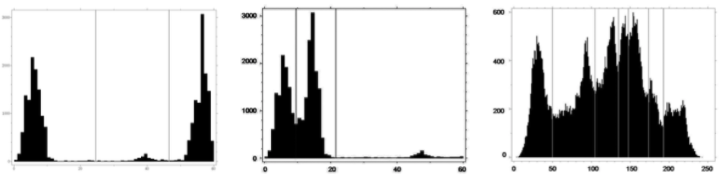
\includegraphics[width=0.48\textwidth]{img/unimodal.png}
\caption{Beispiele der Segmentierung eines Histograms in unimodale Abschnitte. (Quelle: \citep{acopa})}
\label{fig:unimodal}
\end{figure}

Das Histogramm ist offensichtlich in jedem Segment unimodal, wenn $s$ mit den Minima des Histograms initialisiert wird. Es wird nun versucht, Elemente aus $s$ zu entfernen, indem für $\forall i = 1 .. k$ überprüft wird, ob $h$ im Intervall $[h_{s_{i-1}}, \ldots,  h_{s_{i+1}}]$ die \glqq unimodale Hypothese\grqq  erfüllt. Anschaulich bedeutet das die Verschmelzung benachbarter Segmente, so dass das neu entstandene Segment nach wie vor \glqq annähernd unimodal ist\grqq. Hierfür stellen die Autoren in einer separaten Veröffentlichung \citep{ftc} einen parameterfreien statistischen Test vor, der $h$ im betrachteten Intervall mit einem Referenz-Histogramm $h^r$ vergleicht. $h^r$ ist in $[h^r_{s_{i-1}}, \ldots,  h^r_{s_{i+1}}]$ zunächst streng monoton wachsend und danach streng monoton fallend und damit in jedem Fall unimodal. Das Referenz-Histogramm wird aus dem Original-Histogramm $h$ durch Anwendung des Grenander-Operators gebildet. Die komplexen Details hierzu sind \citep{acopa, ftc} zu entnehmen. Da der parameterfreie Test verhältnismäßig aufwändig ist, wird in der eigenen Implementierung auf einen simplen T-Test zurückgegriffen. Dieser liefert ebenfalls befriedigende Ergebnisse, ist aber abhängig vom gewählten Signifikanzniveau.

Das Verfahren zur Histogramm-Segmentierung wird in \citep{ftc} als \textbf{Fine-to-Coarse (FTC) Segmentation Algorithm} zusammengefasst. Zunächst wird $s$ mit allen Minima des Histogramms initialisiert. Daraufhin werden so lange benachbarte Segmente durch Überprüfung der unimodalen Hypothese verschmolzen, bis keine Verschmelzung mehr möglich ist. Die Repräsentanten eines Segments werden durch Mittelung der Samples gebildet, die zum jeweiligen Segment gehören. Abbildung \ref{fig:h_segmentation} zeigt dies an einem Beispiel.

\begin{figure}[h]
\centering
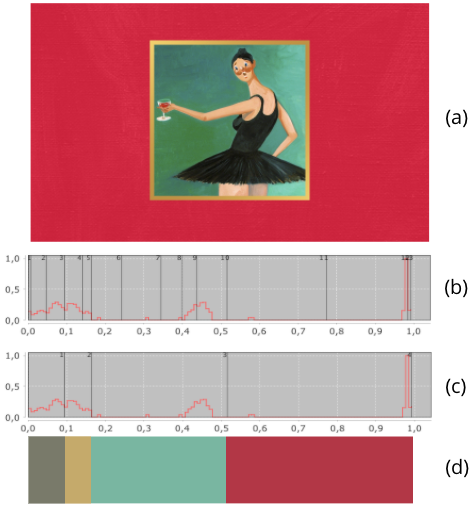
\includegraphics[width=0.48\textwidth]{img/h_segmentation.png}
\caption{Beispiel für eine Segmentierung des Hue-Histogramms. (a) Ausgangsbild, ein Albumcover  von Kanye West. (b) Hue-Histogram (normalisiert), mit allen Minima als initiale Segmentierung. (c) Segmentierung nach Anwendung des FTC Algorithmus. (d) Farbmittelpunkte entsprechend der Samples der jeweiligen Segmente.}
\label{fig:h_segmentation}
\end{figure}

\subsection{Bildung der hierarchischen Farbpalette}

Der ACoPa Algorithmus besteht aus einer hierarchischen Anwendung der Histogram-Segmentierung. Dabei wird zuerst der $h$-, danach der $s$- und abschließend der $i$- Kanal segmentiert. Dabei werden in jedem Schritt die Samples der entstandenen Segmente separiert und die Histogramme der nächsten Ebene getrennt berechnet. Das Ergebnis ist eine hierarchische Farbpalette. Abbildung \ref{fig:palette} zeigt dies am Beispiel der Covers aus Abbildung \ref{fig:h_segmentation}. Auf oberster Ebene (h) wurden die grundsätzlichen Farbtöne des Bildes identifiziert. Auf der zweiten Ebene werden die Farbtöne jeweils in unterschiedliche Sättigungen aufgeteilt, wenn nötig. Auf der dritten Ebene (i) werden von den Sättigungen zusätzlich Helligkeitsabstufungen gebildet.

Die letzte Ebene (i) bildet die Obermenge der Farben $C_s$ für die weitere Verarbeitung. Die Farbpalette spiegelt die in Abschnitt \ref{sec:swatches} definierten Color Swatches wieder. \citet{acopa} empfehlen zusätzlich, die erhaltenen Farben als Startpunkte für den K-Means Algorithmus zu verwenden. Abbildung \ref{fig:palette} (b) zeigt, wie sich die Farben durch K-Means geändert haben. Es ist zu einem späteren Zeitpunkt zu entschieden, welche der beiden Paletten für die weitere Verarbeitung geeigneter ist.

\begin{figure}[h]
\centering
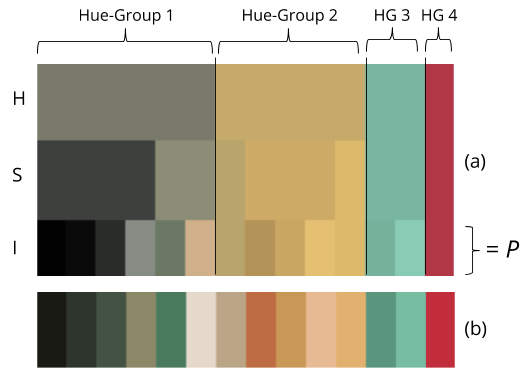
\includegraphics[width=0.48\textwidth]{img/palette.png}
\caption{(a) Hierarchische Farbpalette des Covers aus Abbildung \ref{fig:h_segmentation}. (b) Farbpalette nach Anwendung von K-Means.}
\label{fig:palette}
\end{figure}

\section{Ausblick}

Als nächstes sind die Eigenschaften und Bedingungen der Farben zu ermitteln, die auf der Weboberfläche zum Einsatz kommen sollen. Die Anforderungen müssen in Constraints übersetzt werden. Daraufhin ist ein Algorithmus auszuwählen und zu implementieren, der aus der Farbpalette, die durch ACoPa ermittelt wurde, die passenden Farben herausfiltert. Abschließend werden die Ergebnisse an einer prototypischen Weboberfläche demonstriert.

\bibliographystyle{plainnat}
\footnotesize{\bibliography{references}}

\end{document}
